%-----------------------------------------------%
% Modelo de Plano de Aula com três momentos pedagógicos
%
% Autor: Rodrigo Nascimento (2022-08-12)
%-----------------------------------------------%

\documentclass[
% -- opções da classe memoir --
12pt,				% tamanho da fonte
openright,			% capítulos começam em pág ímpar (insere página vazia caso preciso)
oneside,			% twoside para impressão em verso e anverso. Oposto a oneside
a4paper,			% tamanho do papel. 
% -- opções da classe abntex2 --
chapter=TITLE,		% títulos de capítulos convertidos em letras maiúsculas
%section=TITLE,		% títulos de seções convertidos em letras maiúsculas
%subsection=TITLE,	% títulos de subseções convertidos em letras maiúsculas
%subsubsection=TITLE,% títulos de subsubseções convertidos em letras maiúsculas
% -- opções do pacote babel --
english,			% idioma adicional para hifenização
%	french,				% idioma adicional para hifenização
%	spanish,			% idioma adicional para hifenização
brazil				% o último idioma é o principal do documento
]{abntex2}
\selectlanguage{brazil}
%-----------------------------------------------%
% Informações do DOCUMENTO
%-----------------------------------------------%
\instituicao{Universidade do Estado de Santa Catarina -- UDESC}
\titulo{Estágio Curricular Supervisionado -- IV}
\autor{Rodrigo Nascimento}
\local{Joinville - SC}
\data{\mydate}
\tipotrabalho{Plano de Aula}
\orientador{Prof(a). Dr(a). Ana P. Grimes de Souza}
\coorientador{Prof. Me. Mário Heleno Calegari}
%-----------------------------------------------%
% Para alterar o parâmetros dos comandos orientador
% e coorientador.
%-----------------------------------------------%
% \renewcommand{\orientadorname}{Orientadora:}
\renewcommand{\coorientadorname}{Supervisor:}
%-----------------------------------------------%

\newcommand{\centro}{Centro de Ciências Tecnológicas -- CCT }
\newcommand{\departamento}{Departamento de Física -- DFIS}
\newcommand{\curso}{Licenciatura em Física }
\newcommand{\disciplina}{Estágio Curricular Supervisionado IV-- ESC4003}
\newcommand{\firstkey}{Estágio Supervisionado}
\newcommand{\secondkey}{Ensino de Física}
\newcommand{\thirdkey}{Ensino Médio}


%-----------------------------------------------%

%	Todas as indicações de pacotes e configurações estão no arquivo de estilo
%  chamado texmodel-udesc.sty.
\usepackage{texmodel-udesc}

%-----------------------------------------------%
% Estilo de cabeçalho que só contém o número da 
% página e uma linha
%-----------------------------------------------%
\makepagestyle{cabecalholimpo}
\makeevenhead{cabecalholimpo}{\thepage}{}{} % páginas pares
\makeoddhead{cabecalholimpo}{}{}{\thepage} % páginas ímpares
%\makeheadrule{cabecalholimpo}{\textwidth}{\normalrulethickness} % linha
%-----------------------------------------------%

%-----------------------------------------------%
% HEADER
%-----------------------------------------------%
\begin{document}

\thispagestyle{empty}
\begin{center}
	\begin{minipage}[!]{\linewidth}
		\begin{minipage}[!]{.19\linewidth}
			
\includegraphics[width=\linewidth]{img/logo.png}           
		\end{minipage}
		\begin{minipage}[!]{.8\linewidth}
			\center
			\ABNTEXchapterfont\normalsize\MakeUppercase{\imprimirinstituicao}
			\par
			\vspace*{10pt}                     
			\ABNTEXchapterfont\normalsize\MakeUppercase{\centro}
			\par
			\vspace*{10pt}           
			\ABNTEXchapterfont\normalsize\MakeUppercase{\disciplina}
		\end{minipage}        
	\end{minipage}
	\\ \vspace{0.5cm}
	\rule{\textwidth}{.5pt}   
\end{center}
%-----------------------------------------------%
% Ficha de Identificação
%-----------------------------------------------%
\textual
\begin{center}
	\textbf{A Atmosfera como um Gás Ideal}
\end{center}
\par\noindent\textbf{Estagiário(a):} \imprimirautor\hfill{}\textbf{Orientadora:} Prof(a). Ana Paula Grimes
\par\noindent\textbf{U.E.:} EEB Giovani P. Faraco\hfill{}\textbf{Supervisor:} Prof. Mário Calegari
\par\noindent\textbf{Série:} 2º Ano\hfill{}\textbf{Turma:} Nº(6)
\par\noindent\textbf{Aula:} 007/008\hfill{}\textbf{Data:} 26/04/2023\hfill{}\textbf{Duração:} $2\times 40\min$
\rule{\textwidth}{.5pt}
%-----------------------------------------------%
% Início do Plano de Aula
%-----------------------------------------------%
\bigskip{}  
\noindent
\begin{center}
	\textbf{Entendendo a Equação de Estado do Gás Ideal}
\end{center}
\par\noindent\textbf{Resumo da aula:} Nesta aula será apresentado o modelo de Gás Ideal como uma alternativa à modelagem dos fenômenos atmosféricos. Como recurso didático, utilizar-se-á as simulações interativas do projeto \textit{PhET} da Universidade do Colorado, onde pretende-se mostrar as relações entre as variáveis termodinâmicas $P$, $V$, $n$ e $T$ ao fixar-se uma delas e fazer-se variar as outras. Uma sequência de slides foi desenvolvida para auxiliar na revisão e sistematização desta e das próximas aulas.
\par\noindent\textbf{Habilidades BNCC:} EM13CNT102

\section{Objetivo de Aprendizagem}
\begin{itemize}
	\item Conceber a relação entre a pressão e o volume de uma coluna de ar como um caso particular da Lei de Boyle;
	\item Conceber a relação entre o volume e a temperatura da atmosfera como um caso partícular da Lei de Charles;
	\item Conceber a relação entre o volume e a quantidade de ar atmosférico como um caso particular da Lei de Gay-Lussac.
\end{itemize}

\medskip{}

\noindent\textbf{Núcleo Conceitual:} \emph{Modelagem; Lei dos Gases Ideais; Equação de Estado.}
\newpage

\section{Procedimento Didático} 
% --------------------------------------------- %
\par\noindent\emph{1º Momento:} Revisão
\par\noindent\rule{.3\textwidth}{.5pt}  
\par\noindent\textbf{Tempo previsto:} 20 minutos

\noindent\textbf{Dinâmica:} Revisar os conceitos das últimas aulas a fim de fornecer aos alunos faltantes o suporte necessário para a entendimento da etapa de simulação. Usar a sequência de slides preparada da página 01 até a 17.

Os principais conceitos a serem revisados são
\begin{enumerate}[label=\alph *)]
	\item A temperatura do ar altera as propriedades termodinâmicas de uma coluna de ar, como por exemplo a pressão;
	\item A mudança de pressão em uma coluna de ar, gera forças gradientes de pressão horizontais primeiramente em altitudes e posteriormente em superfícies;
	\item Gradientes de pressões geram ventos sempre em direção à regiões de baixa pressão para compensar o desequilíbrio de pressões.
\end{enumerate}

Avisar aos alunos que a partir de agora iremos investigar estes efeitos a partir de uma simulação, para entendermos melhor como funciona as principais variáveis que descrevem o fenômeno e como elas se interrelacionam.
% --------------------------------------------- %
\vspace{50pt}
\par\noindent\emph{2º Momento:} Simulação
\par\noindent\rule{.3\textwidth}{.5pt}    
\par\noindent\textbf{Tempo previsto:} 30 minutos

\noindent\textbf{Dinâmica:} Abrir a simulação adicionar partículas leves e pesadas, esperar a pressão se estabilizar e fixar a temperatura. A tela da simulação deve parecer-se com a \autoref{fig:pvnrt-pv} a seguir
\setlength\intextsep{0pt}
\begin{wrapfigure}[8]{l}{0.5\textwidth}
	\centering
	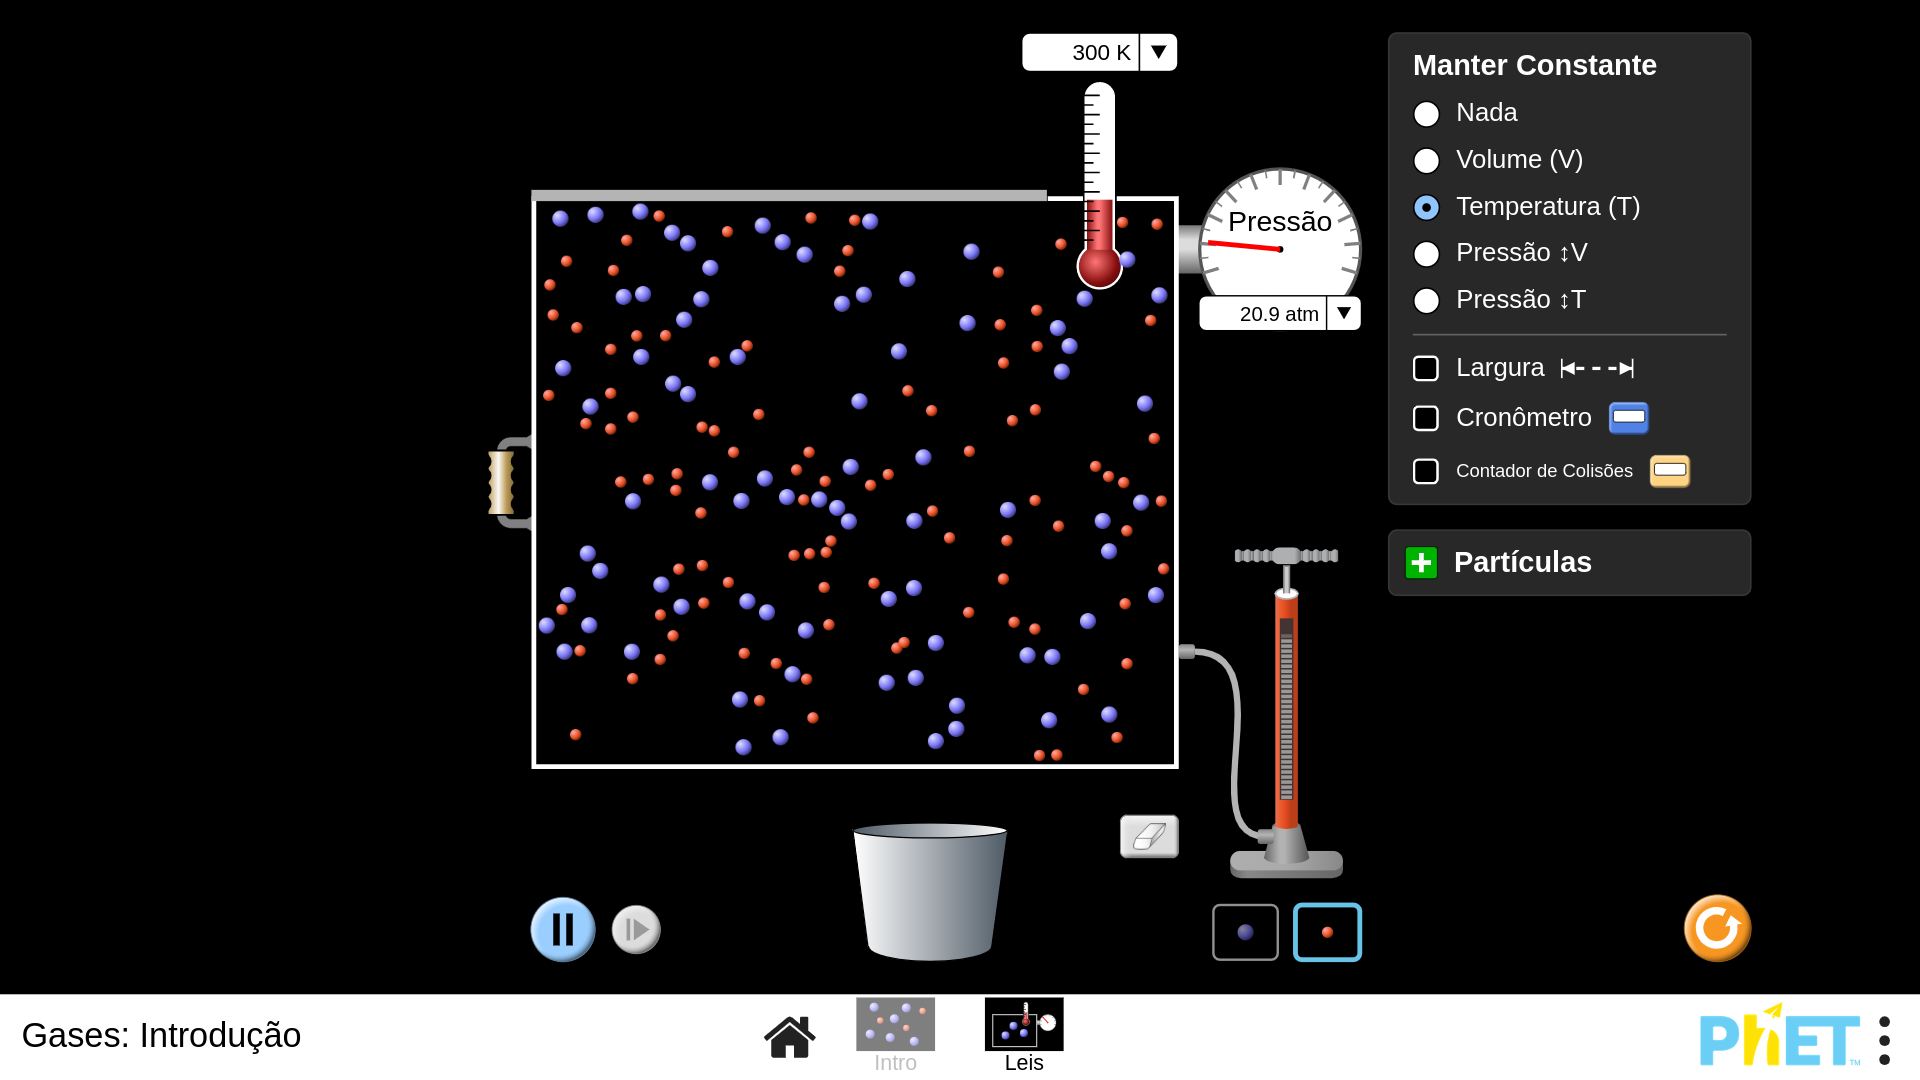
\includegraphics[width=.5\textwidth]{img/pvnrt-pv.png}
	\caption{Simulação Gás Ideal $P \times V$}
	\label{fig:pvnrt-pv}
\end{wrapfigure}
Pedir para que façam previsões do que deve ocorrer com a pressão a medida que se altera o volume do recipiente na simulação. Se possível tentá-los fazer argumentar em favor de suas hipóteses.

Proceder com a simulação aumentando o volume do recipiente e pedindo para que observem o que ocorre com a pressão.

Verificar se as hipóteses dos alunos se confirmaram e discutir os efeitos da mudança de pressão em decorrência do volume. Algum aluno mais atento, pode questionar sobre os resultados desta etapa, uma vez que no estudo atmosférico em questão, a coluna de ar de baixa pressão, encontra-se mais expandida que a sua vizinha mais próxima, no entanto, neste caso o que está ocorrendo não é uma expansão a temperatura constante e sim a pressão constante. A pressão total de ambas as colunas é a mesma, porém há um desequilíbrio de pressão entre a(s) coluna(s) de ar da vizinhança em decorrência da altura do geopotencial de cada uma.

Executar os mesmos procedimentos com as outras variáveis sempre fixando uma, variando as outras e questionando o que esperam que ocorra.
% --------------------------------------------- %
\vspace{50pt}
\par\noindent\emph{3º Momento:} Sistematização
\par\noindent\rule{.3\textwidth}{.5pt}
\par\noindent\textbf{Tempo previsto:} 30 minutos

\par\noindent\textbf{Dinâmica:} Continuar na sequência de slides a partir da pág. 14. Uma vez que obtiveram de forma qualitativa a relação entre as variáveis envolvidas, busca-se agora obter uma relação quantitativa que nos permita estender estes conceitos a qualquer tipo de gás. Para tanto, o professor deve apresentar a Lei de Boyle, Charles e Gay-Lussac de forma discursiva, buscando relacioná-las com as observações feitas na simulação, como exemplo de dicurso podemos ter o seguinte:

\begin{itemize}
		\item "Percebam que quando aumentamos ou diminuimos o volume lá na simulação, a pressão se alterou de forma contrária, dizemos que a pressão é uma grandeza inversamente proporcional ao volume contido de um gás, quando a sua temperatura é mantida constante."
\end{itemize}

Proceder de forma idêntica, passando por todas as situações abordadas na simulação.

Ao final, deve sintetizar com a equação de estado do gás. Uma estratégia para que os alunos não se percam durante esta passagem é escolher uma das grandezas $P$ ou $V$ para ser analisada em toda a exposição e só quando estiver na forma, por exemlo
\begin{align}
		V\propto \frac{1}{P}Tn
\end{align}
reorganizá-la e argumetar a introdução da constante dos gases ideais $R$ a fim de ajustar a igualdade e as unidades de medida. A forma final deve ser a que usalmente é encontrada em qualquer texto do assunto, a saber
\begin{align}
	PV&=nRT
\end{align}

Finalizar a aula na página 17 dos slides, justificando a leve alteração que os meteorologistas fazem na equação de estado, introduzindo a densidade da atmosfera no lugar do número de partículas $n$, ficando assim:
\begin{align}
		P = \rho RT
\end{align}


% --------------------------------------------- %
% Referências
% --------------------------------------------- %
% \bibliography{bibliografia.bib}
% --------------------------------------------- %
% Anexos
% --------------------------------------------- %
\begin{anexosenv}		    
	\chapter{Slides}
	Esta aula conta com uma apresentação em slides como recurso de didático, esta apresentação contém exatas 17 lâminas que podem ser consultadas nas páginas a seguir.
	\includepdf[pages={1-22},nup=2x5]{beamer.pdf}
\end{anexosenv}
% --------------------------------------------- %
% Fim do Plano de Aula
% --------------------------------------------- %
\end{document}
